\begin{figure}[t]
\centering
\definecolor{rankup}{HTML}{1B9E77}\definecolor{rankdown}{HTML}{B5294E}% Rank colors in (c)
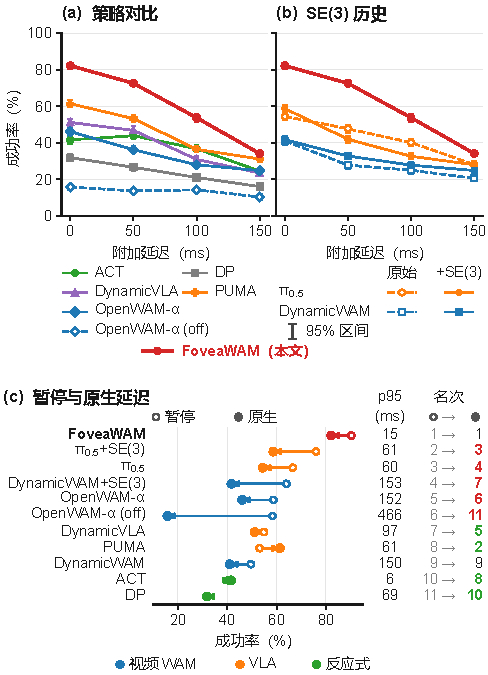
\includegraphics[width=3.25in]{latency/latency_zh.pdf}
\caption{\textbf{\bench 上的延迟。}(a, b) 在各方法原生延迟之上附加延迟时的 SR，分别比较全部策略（a）和原始与 +SE(3) 版本（b）。off：关闭缓存与编译。误差棒：95\% 置信区间。(c) 暂停世界和原生延迟下的 SR，按方法类别着色（同图~\ref{fig:teaser}），各行按暂停名次排列。名次：暂停$\to$原生（2$\to$3 即由第 2 名变为第 3 名）；{\color{rankup}$\blacktriangle$}/{\color{rankdown}$\blacktriangledown$}：上升/下降。}
\label{fig:latency}
\end{figure}
